\documentclass[twocolumn,10pt,a4j]{ltjsarticle}
\usepackage{kougai}

\title{研究報告}
\author{2132100 中野 星花  指導教員 須田 宇宙 准教授}
\date{}

\begin{document}

\maketitle

\section{はじめに}
国際目標であるSDGsに「質の高い教育をみんなに」という目標がある.これを受けて文部科学省は,学習への興味・関心を持ち,協働・対話を通じて自己の考えを広げ深めるという主体的・対話的学習を掲げている.この学習方法では,学習者が自ら考え,他者との意見交換や質疑応答を行うプロセスを通じて,知識の定着や応用力の向上に効果的である.

他者との質疑応答では,教わった人だけではなく教えた人も学習に対する理解が深まることがある.その要因としては,教える過程で自分が持っている知識が整理される点と,相手からの質問や反応を受け取ることで,自分の知識の浅い部分や誤解していた点が明らかになるからである.しかし,質問の仕方が適切ではないと,自分が持っている知識をただ教えるだけになってしまい,教える側の理解力の向上に繋がらないことが問題である.

そこで本研究では,教えることによる学習効果に着目し,教える側の理解が深まる質問方法を挙げ,有用性を検証することを目的とする.

\section{学習について}
一般的に学習する際,講義を受けたり書籍を読むといった受動的な学習活動よりも,知識のアウトプットが伴う活動の方が学習定着率が高いとされている.特に,グループディスカッションや他人に教えることは,その効果がより期待できる.まず,受動的な学習では,知識を得ることは出来ても,実際にその知識を自分の言葉で説明したり応用したりする機会は限られている.そのため,学習内容が短期間で忘れてしまうことが多い.一方,知識のアウトプットを伴う活動では,他人との意見交換やディスカッションを通じて,自身の理解が深まるだけでなく,新たな知識や洞察を得ることができる.これらの活動では,学んだ知識を具体的な問題に応用することが求められるため,単なる暗記にとどまらない深い理解が促される.従って,学習内容の定着率を高めるためには,知識をアウトプットする機会を設けることが必要である.

\section{研究の構想}
他人に教えるという学習には,質問内容が教わる側の知識量に依存してしまう.従って,教える対象をAIにすることで,AIが適切な質問をすることが出来れば,教える側の理解が深まると考えている.

そこで,本研究では,対話形式の他者説明において,学習者が知識を整理し,より理解が深まるような質問内容やシナリオの考案を目的とする.会話形式の他者説明の手法を図1に示す.また,学習者の回答に対する質問内容を簡潔に表1に示す.学習者の回答にもとづく質問内容を分類することで,目標とする理解を促進させるようなシナリオになると考えた.
また,このシステムの対象者によって質問内容の難度が変わる点も考慮する必要があると考えた.

\begin{figure}[h]
\begin{center}
 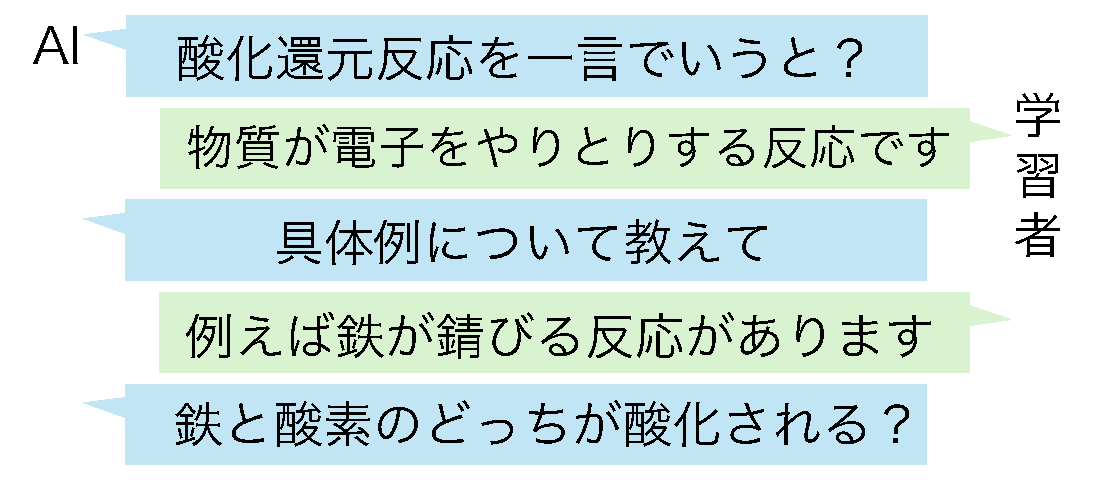
\includegraphics[clip,width=55mm,height=40mm]{talk_log.pdf}
\end{center}
 \caption{対話形式の他者説明}
 \label{fig:図形}
\end{figure}


\begin{table}[h]
\begin{center}
\label{tab:hogehoge}
\begin{tabular}{ll}

\hline

        \multicolumn{1}{l}{学習者の回答} & \multicolumn{1}{l}{質問方法}  \\  \hline \hline 
        \multicolumn{1}{l}{間違いは言っていない} & \multicolumn{1}{l}{具体例を質問} \\ 
         \multicolumn{1}{l}{} & \multicolumn{1}{l}{回答から質問} \\ 
          \multicolumn{1}{l}{} & \multicolumn{1}{l}{まだ聴いてないことを質問} \\ 
          \multicolumn{1}{l}{} & \multicolumn{1}{l}{間違いを再確認} \\ \hline
          \multicolumn{1}{l}{間違いを含む} & \multicolumn{1}{l}{間違った単語を質問} \\
          \multicolumn{1}{l}{} & \multicolumn{1}{l}{聞き返す} \\ \hline
           \multicolumn{1}{l}{間違っている,答えられない} & \multicolumn{1}{l}{回答から質問} \\
          \multicolumn{1}{l}{} & \multicolumn{1}{l}{関連ワードを質問} \\ 
          \multicolumn{1}{l}{} & \multicolumn{1}{l}{説明} \\ \hline
                 
\end{tabular}
\end{center}
\caption{表のタイトル}
\end{table}

\section{今後の予定}
表1をもとに被験者に他者説明をさせ、この質問方法が有効かどうか検証する.





\begin{thebibliography}{99}
\bibitem{suda2018} 須田宇宙: ``音響科学e-Learning教材'', \url{https://www.sudalab.net/}, 2018/7/19参照
\end{thebibliography}

\end{document}
